\chapter{Special Topic: Misc. Physics}\label{ap:spec_phys}
This chapter is a collection of miscellaneous physics topics that I
found interesting. I found the sections to be too short to be
chapters in their own right. In the future, they could be expanded
into chapters, or incorporated into already existing chapters.
Section~\Ref{sec:isohyper} follows Chapter~9 of 
Thomson~\cite{thomson_modern_2013}. 
Section~\Ref{sec:ssb} follows Section~11.1 of Peskin and 
Schroeder~\cite{peskin_introduction_1995}.
Section~\Ref{sec:cscont} follows Chapter 7 of Gattringer and 
Lang~\cite{gattringer_quantum_2010}. 

\section{Isospin and hypercharge}\label{sec:isohyper}
\index{hypercharge}\index{isospin}
In quantum mechanics you learn that spin is a quantum number of
charged particles. For example the electron is a spin-1/2 particle. The
$z$-component $S_3$ of the spin operator $S$ commutes with the Hamiltonian, and
you learn that the eigenvectors of $S_3$ are the +1/2 and -1/2 states. You also
learn that the components of $S$ are related to the Pauli matrices by
\begin{equation}
  S_i=\frac{\hbar}{2}\sigma_i.
\end{equation}

Early on in nuclear physics, scientists noticed that the proton and neutron had
about the same mass, and that the nuclear force between two nucleons (i.e.
protons or neutrons) was approximately charge independent. Therefore Heisenberg
suggested that protons and neutrons were two states of a single particle (the
nucleon) just as there are spin-up and spin-down states of a spin-1/2
particle.
The quantum number corresponding to this property is called {\it isospin}.
Using this idea, the proton and neutron form an isospin doublet with total
isospin $I=1/2$ and $z$-component $I_3=\pm1/2$. Thus the Pauli matrices also
give a suitable representation of the isospin operator, and we write
\begin{equation}
  I^2=\sum\limits_{i=1}^3 I_i^2, \qquad I_i=\frac{1}{2}\sigma_i.
\end{equation}
I know this is sloppy, but I want to leave it to the reader to determine from
context whether $I$ represents the operator or the eigenvalue. 

The concept of isospin can be extended in the same way to quarks. 
In the simplest case we have $N_f=2$ and consider the lightest quarks
$u$ and $d$. The $\SU(2)$ isospin symmetry is only approximate because 
the $u$ and $d$ quarks have slightly different masses. The isospin 
doublet then has a $u$ component and a $d$ component. Generally with
$N_f$ flavors of fermion, the symmetry group is $\SU(N_f)$ and we
form $N_f$ component multiplets in flavor space, one component per flavor.

Let's introduce the $s$ quark and do the $N_f=3$ case.
Using the Pauli matrices and the fact that $\SU(3)$ has 8 generators, you can
figure out what the Gell-Mann matrices are. We will say that $u$, $d$, and $s$
are eigenvectors of isospin and write
\begin{equation}
  u=\colvec{3}{1}{0}{0}, \qquad
  d=\colvec{3}{0}{1}{0}, \qquad
  s=\colvec{3}{0}{0}{1}.
\end{equation}
Then $u$ and $d$ span a 2D subspace of flavor space, so from the earlier
discussion we should know that the generators of $\SU(2)$ are contained in the
generators of $\SU(3)$. Hence
\begin{equation}
  \lambda_1=\left(\begin{array}{ccc}
            0 & 1 &  \\
            1 & 0 &  \\
              &   & 0
            \end{array}\right), \qquad
  \lambda_2=\left(\begin{array}{ccc}
            0 & -i &  \\
            i & 0  &  \\
              &    & 0
            \end{array}\right), \qquad
  \lambda_3=\left(\begin{array}{ccc}
            1 & 0  &  \\
            0 & -1 &  \\
              &    & 0
            \end{array}\right).
\end{equation}
But there's nothing special about $u$ and $d$; $u$ and $s$ will similarly form
a subspace, and so will $d$ and $s$. In both cases, we will use the Pauli
matrices as generators. We can similarly write
\begin{equation}
  \lambda_4=\left(\begin{array}{ccc}
            0 &   & 1\\
              & 0 &  \\
            1 &   & 0
            \end{array}\right), \qquad
  \lambda_5=\left(\begin{array}{ccc}
            0 &    & -i \\
              & 0  &    \\
            i &    & 0
            \end{array}\right), \qquad
  \lambda_X=\left(\begin{array}{ccc}
            1 &    & 0 \\
              & 0  &   \\
            0 &    & -1
            \end{array}\right),
\end{equation}
\begin{equation}
  \lambda_6=\left(\begin{array}{ccc}
            0 &   &  \\
              & 0 & 1\\
              & 1 & 0
            \end{array}\right), \qquad
  \lambda_7=\left(\begin{array}{ccc}
            0 &    &   \\
              & 0  & -i\\
              & i  & 0
            \end{array}\right), \qquad
  \lambda_Y=\left(\begin{array}{ccc}
           0  &    &  \\
              & 1  & 0\\
              & 0  & -1 
            \end{array}\right).
\end{equation}
Finally note the fact that there are only 8 linearly independent generators, so
two of these matrices should be linearly dependent. Since the
$u\leftrightarrow d$ isospin symmetry is the closest to being exact, we choose
the last generator to be a linear combination of $\lambda_X$ and $\lambda_Y$
that treats the $u$ and $d$ quarks symmetrically. Thus
\begin{equation}
  \lambda_8=\frac{1}{\sqrt{3}}\lambda_X+\frac{1}{\sqrt{3}}\lambda_Y
           =\frac{1}{\sqrt{3}}\left(\begin{array}{ccc}
            1 &   &   \\
              & 1 &   \\
              &   & -2
            \end{array}\right).
\end{equation}
The new isospin and total isospin operators are
\begin{equation}
  I^2=\frac{1}{4}\sum\limits_{i=1}^8 I_i^2, \qquad I_i=\frac{1}{2}\lambda_i.
\end{equation}

In the case of $\SU(2)$, the operators $I_i$ do not commute, and therefore are
not simultaneously diagonalizable. For $\SU(3)$ in the Gell-Mann basis,
$I_3$ and $I_8$ are both diagonal, so they correspond to compatible
observables. The observable we associate with $I_8$ is rescaled as
\begin{equation}
  Y=\frac{1}{\sqrt{3}}\lambda_8,
\end{equation}
and $Y$ is called the {\it hypercharge}.
\begin{theorem}{Gell-Mann-Nishijima Formula}{}
\index{Gell-Mann-Nishijima formula}
  The electric charge Q of a particle is related to its isospin and
  hypercharge by
  \begin{equation*}
    Q=I_3+\frac{1}{2}Y
  \end{equation*}
\end{theorem}
%The Higgs doublet has its hypercharge fixed to $Y=1$. Since the first and
%second components have $I_3=\pm1/2$, respectively, we can deduce from this
%formula that the first component has $Q=1$ and the second component has $Q=0$.

%The fact that $\SU(3)$ is also the symmetry corresponding to color means that
%much of the same discussion above also holds for gluons. Instead of $u$, $d$,
%and $s$, we have the colors red ($r$), green ($g$), and blue ($b$).
%The {\it colorless} state is just the color singlet
%\begin{equation}
%  r\bar{r}+b\bar{b}+g\bar{g}
%\end{equation}
%(up to normalization factors).
%Note that the colorless state is a matrix because the antiparticle bar will
%transpose these vectors, so that this state is a sum of outer products.

\section{Spontaneous symmetry breaking}\label{sec:ssb}
\index{spontaneous symmetry breaking}
Let $\phi(x)$ denote a vector (in the mathematical sense) of $N$ real,
scalar fields $\phi^i(x)$. Then the Lagrangian
\begin{equation}
  \Lagr=\frac{1}{2}\left(\partial_\mu\phi\right)^2
        +\frac{1}{2}\mu^2\phi^2-\frac{\lambda}{4}\phi^4
       \equiv\frac{1}{2}\left(\partial_\mu\phi\right)^2
        +V(\phi)
\end{equation}
is invariant under $O(N)$. (Recall orthogonal transformations are the
ones with $R^TR=\id$.) This is the Lagrangian of the {\it linear
sigma model}. Note that is is a generalization of $\phi^4$ theory,
but we have replaced the positive mass parameter $m^2$ with a
negative parameter $-\mu^2$ and rescaled $\lambda$ to eliminate a factor of 6.
Classically, the potential is minimized when $\phi$ lies
on an $N$-dimensional sphere of radius $\sqrt{\mu^2/\lambda}$, i.e. 
it is minimized for vectors $\phi_\text{min}$ satisfying
\begin{equation}
  \phi_\text{min}^2=\frac{\mu^2}{\lambda}.
\end{equation}
To interpret the theory, we first choose coordinates so that 
$\phi_\text{min}$ lies
entirely along the $N$ direction
\begin{equation}\label{eq:phidir}
  \phi_\text{min}=(0,0,...,0,v),
\end{equation}
where $v=\sqrt{\mu^2/\lambda}$ is the {\it vacuum expectation value} or VEV.
Then, we define a set of shifted fields $\pi_k$ and $\sigma$ relative
to this point by writing
\begin{equation}\label{eq:phishift}
  \phi(x)=\left(\pi_1(x),\pi_2(x),...,\pi_{N-1}(x),v+\sigma(x)\right)
\end{equation}
Written in terms of $\pi$, the $N-1$ dimensional vector with components
$\pi_k$, and $\sigma$, the new Lagrangian becomes
\begin{equation}\label{eq:brokenlagr}
  \Lagr=\frac{1}{2}\left(\partial_\mu\pi\right)^2
        +\frac{1}{2}\left(\partial_\mu\sigma\right)^2
        -\frac{1}{2}\left(2\mu^2\right)\sigma^2-\sqrt{\lambda}\mu\sigma^3
        -\sqrt\mu\pi^2\sigma
        -\frac{\lambda}{4}\sigma^2
        -\frac{\lambda}{2}\pi^2\sigma^2
        -\frac{\lambda}{4}\pi^4,
\end{equation}
where we have removed constant terms, because they do not change the
physics. Equation~\eqref{eq:brokenlagr} is the Lagrangian of $N-1$
massless, dynamic fields $\pi_k$ and a dynamic field $\sigma$ with mass
$\sqrt{2}\mu$. Written in this form, the original $\text{O}(N)$ symmetry
is now obscured. There is a remaining $\text{O}(N-1)$ symmetry
rotating the $\pi_k$ among themselves. This is an example of
{\it spontaneous symmetry breaking} (SSB), and we say something like
``the original $\text{O}(N)$ symmetry spontaneously breaks to
the subgroup $\text{O}(N-1)$." 

\begin{figure}[t]
\centering
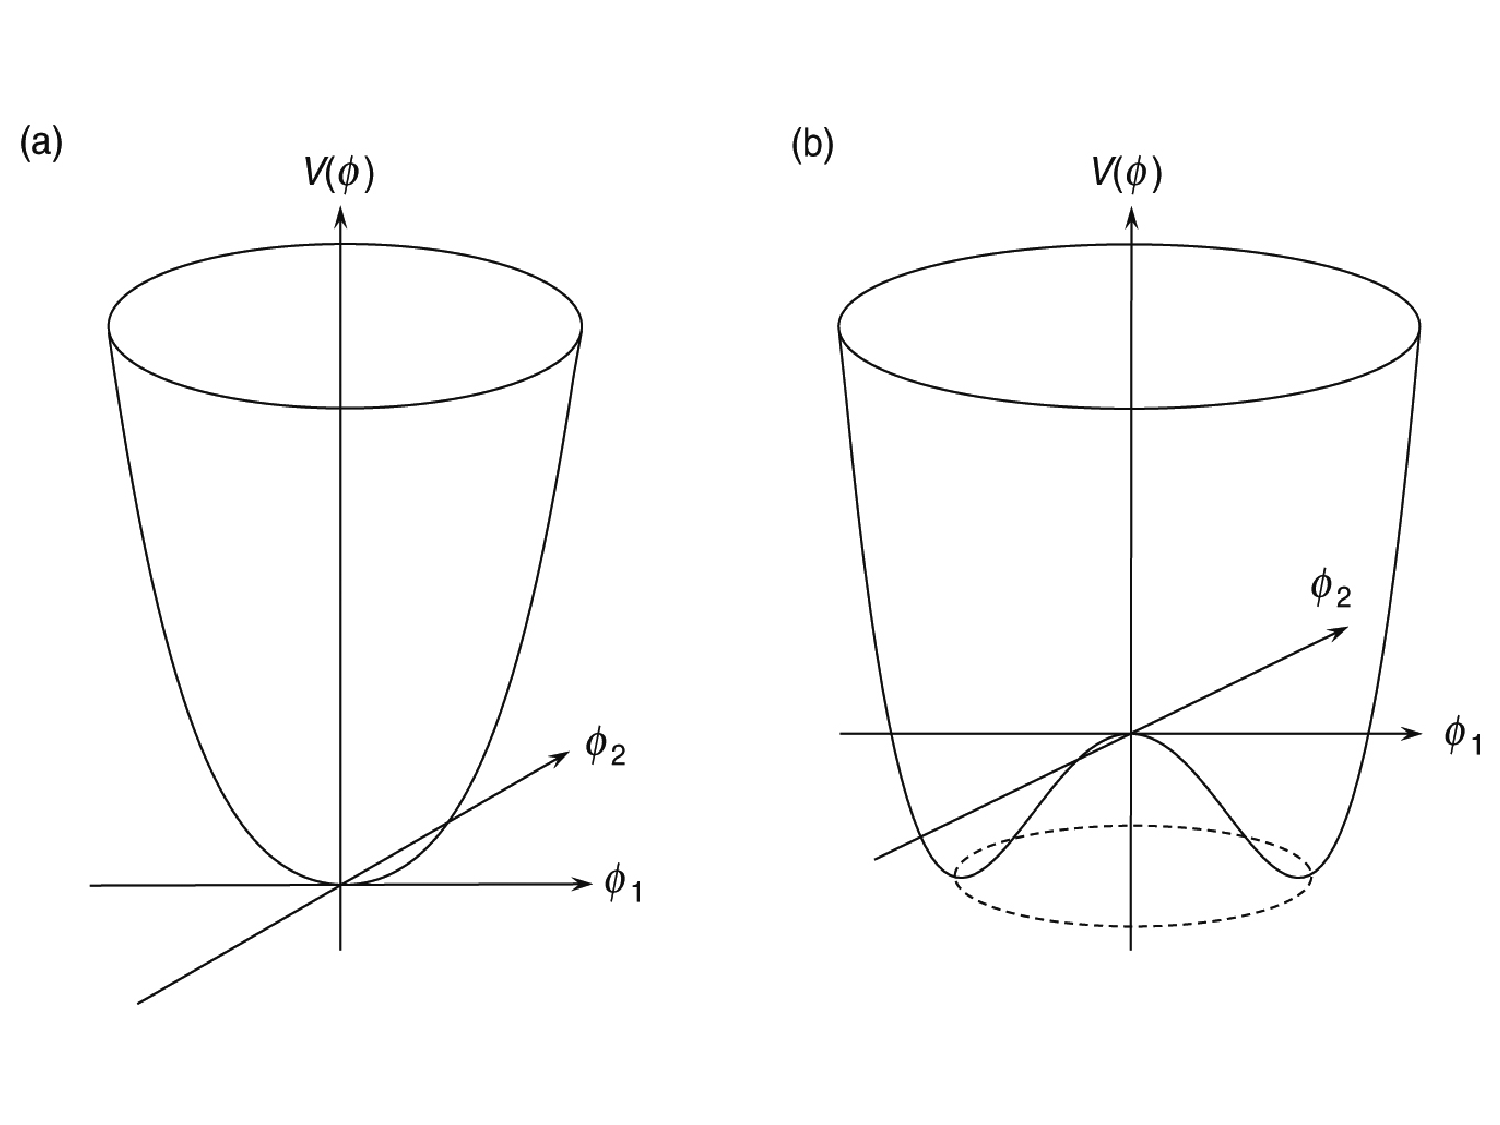
\includegraphics[width=0.8\linewidth]{figs/symm_break.pdf}
\caption{Linear sigma model potential for $N=2$. In (a) the $\phi$ field
         mass term $m^2>0$, while (b) gives this potential when
         $m^2$ is replaced by a negative parameter $-\mu^2$.
         Oscillations along the circle of minima in (b) correspond to 
         the $\pi$ field. Oscillations in the radial direction correspond
         to the $\sigma$ field. Image taken from 
         Thompson~\cite{thomson_modern_2013}.}
\label{fig:ssb}
\end{figure}

Let's try to gain some geometric intuition for this phenomenon. 
Looking at eq.~\eqref{eq:phidir}, we see that in $\phi$ space, the $\sigma$
field corresponds to oscillations of $\phi$ orthogonal to the $N-1$
dimensional hypersurface, while the massless $\pi_k$ fields
corresponds to oscillations along the hypersurface. 
An example with $N=2$ is shown in Figure~\Ref{fig:ssb}. 
If we take the ground state vector~\eqref{eq:phidir} and hit it with
$\text{O}(N)$, it will be rotated somewhere else on the hypersurface.
The subgroup $\text{O}(N-1)$ hits the first $N-1$ components of the
ground state, which are all 0, thereby leaving it unchanged.
In the original $\phi^4$ theory with
$m^2>0$, the ground state vector was 0, so the $\text{O}(N)$ symmetry
was also a symmetry of the ground state. After SSB, $\text{O}(N)$ changes 
the ground state vector in general,
which is why we say the symmetry is broken. Generally any symmetry
respected by the Lagrangian but not by the ground state vector
is a broken symmetry.

In the linear sigma model, massless $\pi$ particles appeared after
SSB. This is a special example of a general result
known as Goldstone's theorem. The generated massless particles are
referred to as \index{Goldstone!boson}{\it Goldstone bosons}. 
Many light bosons can be interpreted
as approximate Goldstone bosons; as we will see in Section~\Ref{sec:cscont},
the pion can be viewed in this manner.
\begin{theorem}{Goldstone's theorem}{}
\index{Goldstone!theorem}
Consider a Lagrangian of the form
$$
  \Lagr=(\text{kinetic term for $\phi$})+
        (\text{terms independent of $\phi$})-V(\phi),
$$
where $\phi$ is the $N$-dimensional vector of real, scalar fields
$\phi_k$, and $\Lagr$ is invariant under a continuous, global
transformation of $\phi$ with generators $T^a$. Then for every
spontaneously broken generator there exists a corresponding
Goldstone boson. 
\begin{proof}
  Let $\phi_\text{min}$ be a constant field minimizing $V$. Expanding
  $V$ about this minimum we get to leading order
  $$
    V(\phi)= V(\phi_\text{min})
     +\frac{1}{2}
      (\phi-\phi_\text{min})_i(\phi-\phi_\text{min})_j\,
      \frac{\partial^2 V}{\partial\phi_i\partial\phi_j}
       \Big|_{\phi=\phi_\text{min}}.
  $$
  The differences $\phi-\phi_\text{min}$ give the new fields of the
  theory after SSB; for example in the linear sigma model this difference
  is, from equations~\eqref{eq:phidir} and \eqref{eq:phishift},
  $$
    \phi-\phi_\text{min}=(\pi_1,...,\pi_{N-1},\sigma).
  $$
  Therefore the coefficient of the quadratic term is a symmetric matrix
  whose eigenvalues give the masses of these fields. If we can prove
  that each broken generator implies a zero eigenvalue for this matrix,
  we are done.
  The kinetic term for $\phi$ is already invariant under the global
  transformation, so if $\Lagr$ is invariant, it follows that $V$ must
  be as well. Then we can write
  $$
    V\left((\id-i\omega^aT^a)\phi\right)=V(\phi),
  $$
  where $\omega$ is some infinitesimal parameter. Expanding to linear
  order yields
  $$
    \frac{\partial V}{\partial\phi_j}(T^a\phi)_j=0.
  $$
  Differentiating the above with respect to $\phi_i$ and evaluating at
  $\phi_\text{min}$ gives
  $$
     \frac{\partial^2 V}{\partial\phi_i\partial\phi_j}
      \Big|_{\phi=\phi_\text{min}}(T^a\phi_\text{min})_j=0,
  $$
  i.e. $T^a\phi_\text{min}$ is annihilated by the mass matrix. 
  If $T^a$ is a broken generator, we have $T^a\phi_\text{min}\neq0$,
  so the above equation implies $T^a\phi_\text{min}$ is an
  eigenvector of the mass matrix with eigenvalue zero.
\end{proof}
\end{theorem}

%In the basis that diagonalizes the mass matrix, the eigenvectors correspond
%to different fields, each with a mass equal to its corresponding eigenvalue.
%
%If you hit the VEV with a broken symmetry, it will rotate it. In the
%$N=2$ linear sigma model, the broken O(2) symmetry rotates the VEV.
%
%Even if it's not clear how the pions in the first case rise from this
%procedure, the important thing is that it guarantees some field
%eigenvectors of M^2, which have 0 eigenvalue. 

\section{Chiral symmetry in the continuum}\label{sec:cscont}
\index{chiral symmetry}

In the continuum, the massless fermion action for a single flavor reads
\begin{equation}
S_F=\int\dd[4]{x}\Lagr_F=\int\dd[4]{x}\bar{\psi}\slashed{D}\psi. 
\end{equation}
We refer to $\slashed{D}$ as the {\it massless Dirac operator}. A 
{\it chiral rotation}\footnote{You may notice that the sign in the exponent
is the same for both the spinor field and its conjugate field. This is a
common feature whenever a $\gamma_5$ is in the exponent. Recall that
$\bar{\psi}=\psi^\dagger\gamma_4$. The $\gamma_5$ will anticommute with 
$\gamma_4$.} of the fermion fields is a transformation
mapping
\begin{equation}
  \psi\to e^{i\alpha\gamma_5}\psi~~~~\text{and}~~~~
  \bar{\psi}\to\bar\psi e^{i\alpha\gamma_5},
\end{equation}
where $\alpha\in\mathbb{R}$. This is probably called a chiral rotation
because $\gamma_5$ is used to define the operators~\eqref{eq:projdef},
which project out the left-handed and right-handed components of the
fermion field according to eq.~\eqref{eq:projact}. Using identity 2 of
Proposition~\Ref{prp:gammatech}, we find that $\Lagr_F$ transforms under this
rotation as
\begin{equation}
  \Lagr_F\to\bar{\psi}e^{i\alpha\gamma_5}\slashed{D}e^{i\alpha\gamma_5}\psi
         =\bar{\psi}e^{i\alpha\gamma_5}e^{-i\alpha\gamma_5}\slashed{D}\psi
         =\Lagr_F,
\end{equation}
i.e. it is invariant under chiral rotations. Using
Proposition~\Ref{prp:projection}, one can decompose $\Lagr_F$ into its
left-handed and right-handed parts as
\begin{equation}
  \Lagr_F=\bar{\psi}_L\slashed{D}\psi_L
         +\bar{\psi}_R\slashed{D}\psi_R,
\end{equation}
and we colloquially say that the chiral components of
$\Lagr_F$ ``do not talk to each other."
If one were to include a mass term in $\Lagr_F$, it would decompose as
\begin{equation}
  m\bar{\psi}\psi=m\left(\bar{\psi}_R\psi_L+\bar{\psi}_L\psi_R\right),
\end{equation}
which mixes the chiral components, thereby breaking chiral symmetry.
This is why one refers to the limit $m\to0$ as the {\it chiral limit}.

We now generalize these ideas to $N_f$ flavors of fermion. In Gattringer
and Lang eq.~(7.11), they write the fermion action as
\begin{equation}\label{eq:nfact}
  S_F=\int\dd[4]{x}\Lagr_F=\int\dd[4]{x}
         \bar{\psi}\left(\slashed{D}+M\right)\psi,
\end{equation}
where $M$ is the {\it mass matrix}\index{mass matrix}
\begin{equation}
  M~``="~\diag(m_1,m_2,...,m_{N_f})
\end{equation}
acting in flavor space. $M$ cannot be a $N_f\times N_f$ matrix, because
we have defined $\gamma^\mu$ as a $4\times4$ matrix. The only way adding 
these matrices makes sense is if $M$ is a $4N_f\times4N_f$ matrix, i.e. if
\begin{equation}
  M=\left(\begin{array}{cccc}
      m_1\id_4 &          &        & \\
               & m_2\id_4 &        & \\
               &          & \ddots & \\
               &          &        & m_{N_f}\id_4
    \end{array}\right).
\end{equation}
Then $\psi$ must be a $4N_f$ vector (in the mathematical sense, not 
in the Lorentz transformation sense) looking something like
\begin{equation}
  \psi=\colvec{4}{\psi_1}{\psi_2}{\vdots}{\psi_{N_f}},
\end{equation}
where each $\psi_i$ is a 4-component Dirac spinor, and presumably when
we write $\gamma^\mu$ in eq.~\eqref{eq:nfact} what we really mean is
\begin{equation}
  \gamma^\mu=\gamma^\mu\id_{N_f}
            =\left(\begin{array}{cccc}
               \gamma^\mu &            &        & \\
                          & \gamma^\mu &        & \\
                          &            & \ddots & \\
                          &            &        & \gamma^\mu
               \end{array}\right).
\end{equation}
I pray the reader forgives the notational perversion in the above equation.

In the chiral limit, the action eq.~\eqref{eq:nfact} is again invariant under
chiral rotations, also in this context called {\it axial vector rotations},
taking the form
\begin{gather}
  \label{eq:SUNfc}
  \psi\to e^{i\alpha\gamma_5 T^a}\psi,\qquad
    \bar{\psi}\to\bar{\psi}e^{i\alpha\gamma_5 T^a}, \\
  \label{eq:U1A}
  \psi\to e^{i\alpha\gamma_5 \id}\psi,\qquad
    \bar{\psi}\to\bar{\psi}e^{i\alpha\gamma_5 \id},
\end{gather}
where the $T^a$ are the $N_f^2-1$ generators of $\SU(N_f)$,
$\id\equiv\id_{4N_f}$, and again $\alpha\in\mathbb{R}$.
In this limit the action is also invariant under the
{\it vector transformations}
\begin{gather}
  \label{eq:SUNf}
  \psi\to e^{i\alpha T^a}\psi,\qquad
    \bar{\psi}\to\bar{\psi}e^{-i\alpha T^a}, \\
  \label{eq:U1V}
  \psi\to e^{i\alpha \id}\psi,\qquad
    \bar{\psi}\to\bar{\psi}e^{-i\alpha \id}.
\end{gather}
This invariance under the above two equations extends to the case of degenerate
masses, when $m_1=m_2=...=m_{N_f}\equiv m$, and is the familiar isospin
symmetry generalized to $N_f$ flavors. The symmetry~\eqref{eq:U1V} holds for
arbitrary masses, and the conserved quantity is the {\it baryon number}
\begin{equation}
    B=\frac{1}{3}(n_q-n_{\bar{q}}).
\end{equation}
You can see why it's called baryon number: A baryon is made of 3
quarks, and hence has $B=1$. Anti-quarks have $B=-1$, and
mesons have $B=0$.

Returning once again to the massless limit, the invariance of the action under
eqs.~\eqref{eq:SUNfc}, \eqref{eq:U1A}, \eqref{eq:SUNf}, and \eqref{eq:U1V}
represents the global symmetry group
\begin{equation}\label{eq:SMfglobal}
  \SU(N_f)_L\times\SU(N_f)_R\times\U(1)_V\times\U(1)_A.
\end{equation}
Breaking the global symmetry group~\eqref{eq:SMfglobal} has important
implications in QCD phenomonology. For example we will show that in the
quantized, massless theory the fermion determinant changes
under~\eqref{eq:U1A}, breaking the $\U(1)_A$ symmetry explicitly. The remaining
symmetry is
\begin{equation}\label{eq:SMglobalbUA}
  \SU(N_f)_L\times\SU(N_f)_R\times\U(1)_V.
\end{equation}
If the fermion masses are degenerate, the symmetry $\SU(N_f)_L\times\SU(N_f)_R$
breaks to its subgroup $\SU(N_f)_V$. Now the remaining symmetry is
\begin{equation}
  \SU(N_f)_V\times\U(1)_V.
\end{equation}
Finally allowing non-degenerate masses breaks the symmetry further. 
There remains
\begin{equation}
  \underbrace{\U(1)_V\times\U(1)_V\times...\times\U(1)_V}_\text{$N_f$ times}.
\end{equation}

The typical QCD scale is $\sim1~\text{GeV}$ (think protons, which have a 
mass of about 940~MeV) so the $u$, $d$, and $s$ quarks have masses that
are relatively small (about 5~MeV, 5~MeV, and 100~MeV, respectively).
Since these masses are so close to zero on this scale, we can say that
when $N_f=2$, and partly for $N_f=3$, eq.~\eqref{eq:SMglobalbUA} is
an approximate symmetry. If the $u$ and $d$ quarks were massless, this symmetry
would be exact, and it can be argued~\cite{gattringer_quantum_2010} that
a nucleon and its negative parity partner should have the same mass. 
However one finds the negative parity nucleon to have
a mass of about 1535~MeV, and this difference of about 600~MeV is too large to
be explained by the slight breaking due to the $u$ and $d$ masses. We
conclude that something else is happening. This something is called 
{\it spontaneous chiral symmetry breaking}, and it comes out of the
dynamics of QCD. If quarks were massless, the pions would arise as 
the Goldstone bosons of chiral SSB; hence we refer to pions as 
``would-be" Goldstone bosons.

% Berg insight relating this stuff to pure SU(N): in our simulations we sample
% A_\mu, so \partial_\mu + iA_\mu is well defined, which means
% \gamma_\mu(\partial_\mu +iA_\mu) is well defined, which is the Dirac
% operator. The Dirac operator is a matrix, so as long as it's diagonalizable
% you can find eigenvectors. The fact that our action is pure SU(N) only really
% changes the distribution of the A_\mu.
%\section{Chiral symmetry on the lattice}\label{sec:cslat}
%For light quarks, the fermion action is roughly invariant under the global
%symmetry~\eqref{eq:SMglobalbUA}. Experimental findings do not reflect this
%chiral symmetry, so we conclude it is broken spontaneously by QCD dynamics.
%The small pion masses can be attributed to a further, slight breaking
%of this symmetry. Since chiral symmetry breaking is important in high
%energy phenomenology, it is worth implementing on the lattice.

\bibliographystyle{unsrtnat}
\bibliography{bibliography}
